%%% Preamble
  \documentclass[a4paper, 11pt]{article}
  \usepackage[T1]{fontenc}
  \usepackage{fourier}
  \usepackage[english]{babel}
  \usepackage[protrusion=true,expansion=true]{microtype}
  \usepackage{amsmath,amsfonts,amsthm}
  \usepackage[pdftex]{graphicx}
  \usepackage{url}
  \usepackage{setspace}
  \usepackage{vmargin}
  \setmarginsrb {0.79in}  % left margin
                {1.00in}   % top margin
                {0.79in}   % right margin
                {0.79in}  % bottom margin
                {  20pt}   % head height
                {0.25in}   % head sep
                {   9pt}    % foot height
                { 0.3in}    % foot sep

  \usepackage{sectsty}
  \allsectionsfont{\centering \normalfont\scshape}

  % Bibliography
  \usepackage{natbib}
  \bibliographystyle{aer}
  \setlength{\parindent}{0.25in}


  %% Added by me
  \usepackage{pdfpages}
  \usepackage{booktabs}
  \usepackage{wrapfig}
  \usepackage{float}
  \usepackage{pdfsync}
  \usepackage{fancyhdr}
  \usepackage{multicol}
  \newcommand\ve{\varepsilon} % From Rick
  \theoremstyle{definition} % From Rick
  \newtheorem{definition}{Definition} % Number definitions on their own
  \usepackage{hyperref}  % From Rick
  \hypersetup{colorlinks,linkcolor=cyan,urlcolor=blue,citecolor=black}
  \usepackage{colortbl}
  \usepackage{caption}

  %%% Equation and float numbering
  \numberwithin{equation}{section}

  %% EVEYTHING BELOW NEEDS TO BE CHANGED!
  %% Setup default header
  \fancypagestyle{mainDoc}{
      \fancyhead[L]{\small GARCH - ARIMA EPP}
      \fancyhead[R]{\thepage}
      \fancyfoot{} % no footer
      \renewcommand{\headrulewidth}{.5pt}
      \renewcommand{\footrulewidth}{0pt}
      \setlength{\headheight}{13.6pt}
  }

  %%% Maketitle metadata
  \newcommand{\horrule}[1]{\rule{\linewidth}{#1}}     % Horizontal rule

  % Set title here
  \newcommand \thetitle{Risk Analysis Using GARCH and ARIMA Models}

  \title{
    \vspace{-.6in}
    \usefont{OT1}{bch}{b}{n}
    \normalfont \normalsize \textsc{ } \\ [25pt]
    \horrule{0.5pt}
    \huge \thetitle \\
    \horrule{2pt}
  }

  \author{
    Spencer Lyon
    % \thanks{}
  }

  \date{
  \normalfont \normalsize
  \today \\[-4pt] \normalsize
  }

  \newcommand{\TODO}[1]{ {\color{magenta} TODO: #1} }

%% Title Page
\begin{document}
\begin{titlepage}
  \maketitle
  \thispagestyle{empty}
  \begin{center}

  
\includegraphics{logo} \\ [0.8cm] % University/department logo - uncomment to place it

  Macroeconomics and Computational Laboratory (MCL) \\[0.5cm] % Research group name
  BYU Economics\\[1.5cm]  % and department name

  % \large{\textit{Abstract}}
  \begin{abstract}
      \normalsize
      \setstretch{1.75}
        Put an awesome abstract here.
  \end{abstract}
  \end{center}
  \tableofcontents
\end{titlepage}

%% Main document
\newpage
\pagenumbering{arabic}  % Use arabic numbers now
\setcounter{page}{1}  % Reset page numbering

\begin{center}
\huge{\thetitle}  % Make sure the newcommand \thetitle is defined above
\rule{\linewidth}{.1pt}
\end{center}

\setstretch{1.75}

\section{Introduction} \label{sec:intro}
  \thispagestyle{empty}
  \pagestyle{mainDoc}

  One longstanding phenomenon economists see in financial data is known as the equity premium puzzle \citep{Prescott:1985}. The heart of the equity premium puzzle can be summarized one of two equivalent questions: why is demand for risk free government bonds so high when returns on those assets are so low? The second question could be stated as follows:  why is demand for stocks, and hence stock prices, so low despite the relatively high expected returns

  Over the years economists have posed many possible explanations for why the equity puzzle premium (EPP) exists, or even if it exists. Modern economics is based largely on rational expectations and risk aversion. An appeal to these theories to explain the EPP seems natural and intuitive; however, this type of explanation falls very short. To put this disparity in perspective \cite{Mankiw:1991} pointed out that in order for risk aversion to explain the EPP, investors would have to be indifferent between taking a sure \$51,209 or having 50\% at winning either \$50,000 and \$100,000. Other common explanations have generally been rooted in tax policy, market failures, liquidity constraints, and the implied volatility of the underlying equities.

  The focus of this paper will be analyzing the ability of ARIMA and (G)ARCH models for identifying and explaining the equity premium puzzle. ARMIA methods have been around for some time and have held a significant foothold in the finance literature.  An ARIMA model allows the economist to model the effect of historical moving averages on current values. This flexibility is particular appealing to someone trying to model financial time series because things like seasonality, momentum, and market lags and/or inefficiencies lead to these moving averages storing a lot of relevant data.

  ARCH and GARCH models are, in a sense, very similar to ARIMA models. Instead of trying to model the effect of changing moving averages, (G)ARCH models attempt to capture changes in the variance of underlying parameters. It is immediately apparent the trained financial eye that focusing on the changes in expected variance might actually be more instructive than moving averages when applied to forecasting models.

  The remainder of this paper will be structured as follows: Section ~\ref{sec:estimation} will discuss ARIMA and (G)ARCH models as well as the data I am using, Section~\ref{sec:results} will show the results of my analysis, and Section~\ref{sec:conclusion} will have a few concluding thoughts and ideas for further research.

\section{Estimation} \label{sec:estimation}

  \subsection{The Data} \label{sub:the_data}

    The data for this paper is quite simple. To mimic a risk free asset I have gathered daily data for the price of both 3-month and 10-year US treasury bills. I obtained this data from the St. Louis Federal reserve under the data set names DGS3MO and DGS10 for the 3-month and 10-year maturities, respectively. The units on these data sets are percent returns, the data is not seasonally adjusted, and the data was sampled at a daily frequency.

    To model risky assets I chose to use the daily returns on the S\&P 500 stock market index.  The units on this data set is US dollars (\$) and I retrieved the data from Yahoo! Finance. The S\&P 500 was a natural choice because it is a very common metric used in finance to measure the overall movement of the stock market. Because some explaination of the EPP refer to the volatility of stocks I also chose to use the VIX, also from Yahoo! Finance. \footnote{The VIX is constructed using the implied volatilities on call and put options for the stocks making up the S\&P 500. It is the generally accepted measure of overall stock market volatility.}

    For the most part, these four time series had observations on the same days: all of them are reported for week-days only. However, the big difference is that the data from Yahoo! Finance is only reported on trading days, while the data from FRED is reported every Monday through Friday, including most holidays. To overcome this I simply dropped observations for days where FRED reported data, but the stock markets were closed. In Table ~\ref{tab:describe} I have included a summary of this data and a simple plot of the data in Figure ~\ref{fig:alldata}.

    \setstretch{1.2}
    \begin{figure}[ht]
        \centering
        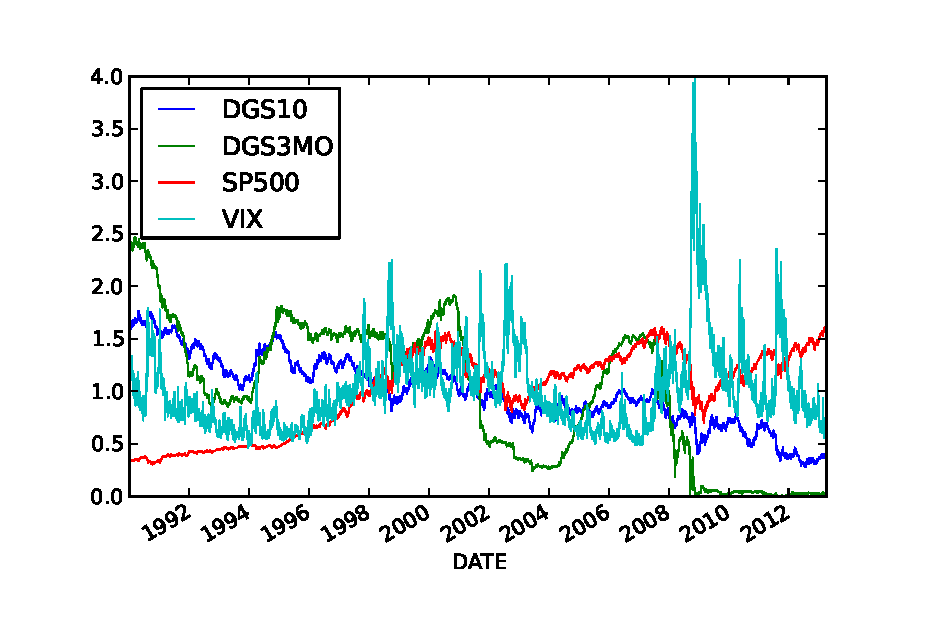
\includegraphics[width=6in]{./Figures/all_data.eps}
        \captionsetup{width=5.5in}
        \caption{\small Plot of the data used in this paper. Note that because the units are different and the value of the S\&P 500 is much larger than the percents on the T-bill data sets, I have divided each data set by its mean before plotting.}
        \label{fig:alldata}
    \end{figure}

    \begin{table}[ht!]
      \begin{center}
        \begin{tabular}{r|ccccc}
        \hline
           \rowcolor{gray!45}  & DGS10  (\%)& DGS3MO  (\%)& SP500 (\$)& VIX (\$)\\
          \hline
          \hline
          \rowcolor{gray!7} obs & $3305$ & $3305$ & $3305$ & $3305$\\
          \rowcolor{gray!23} mean & $3.99311$ & $2.10994$ & $1210.33$ & $21.8055$\\
          \rowcolor{gray!7} std & $1.14046$ & $2.01772$ & $187.527$ & $9.16702$\\
          \rowcolor{gray!23} min & $1.43$ & $0$ & $676.53$ & $9.89$\\
          \rowcolor{gray!7} 25\% & $3.38$ & $0.15$ & $1095.45$ & $15.54$\\
          \rowcolor{gray!23} 50\% & $4.12$ & $1.59$ & $1214.91$ & $20.03$\\
          \rowcolor{gray!7} 75\% & $4.74$ & $3.85$ & $1357.98$ & $25.4$\\
          \rowcolor{gray!23} max & $6.79$ & $6.42$ & $1569.19$ & $80.86$\\
        \bottomrule
        \end{tabular}
        \captionsetup{width=5.5in}
        \caption{\small Summary of the data . All the data was sampled from 1/1/2000 to 3/28/2013. Note the rows with percent labels correspond to percentiles}
        \label{tab:describe}
      \end{center}
    \end{table}
    \setstretch{1.75}

  \newpage
  \subsection{ARIMA Models} \label{sub:arima}

    Time series modeling is all about identifying time-varying trends in data and extrapolating those trends into the future with as little error as possible. One extremely general family of time series models is known as the ARIMA model, or autoregressive integrated moving average model. There are at least three roles an ARIMA model (or any forecasting model) can play:

    \begin{enumerate}
      \item By themselves to predict future values of a dependent variable
      \item To predict the future value of an independent variable in an economic model
      \item To estimate future values of systematic residuals in an economic model
    \end{enumerate}

    In this paper I will be using ARIMA models within the first category listed above. In order to understand how I will be using them I will first explain what the model is in a general form. An ARIMA model is defined in terms of three parameters $p, q, \text{ and }, d$ and is defined as follows:

     \begin{align}
     Y_t^* - \phi_1Y_{t-1}^*  - \dots - \phi_pY_{t-p}^* &= \ve_t - \theta_1\ve_{t-1} - \dots - \theta_q \ve_{t-q} \label{eq:arimalong}\\
     \left( 1 - \sum_{i=1}^p \phi_i L^i\right) Y_t^* &= \left( 1 + \sum_{i=1} ^q \theta_i L^i \right) \ve_t \label{eq:arima}
     \end{align}

    Where $L$ is the lag operator and $Y_t^* \equiv (1 - L)^d Y_t$.

    \subsubsection{Identification} \label{ssub:identification}

      The first major roadblock when trying to build an ARIMA model is identifying the parameters $p, q, \text{ and } d$. I will start by trying to identify $p$ and $q$. To do this I need to look at the autocorrelation and partial autocorrelation coefficients (see McDonald notes section 8). In Figure~\ref{fig:correlations} I have included a plot of the autocorrelation and partial autocorrelation coefficients for each data set.

      \begin{figure}[!h]
        \centering
        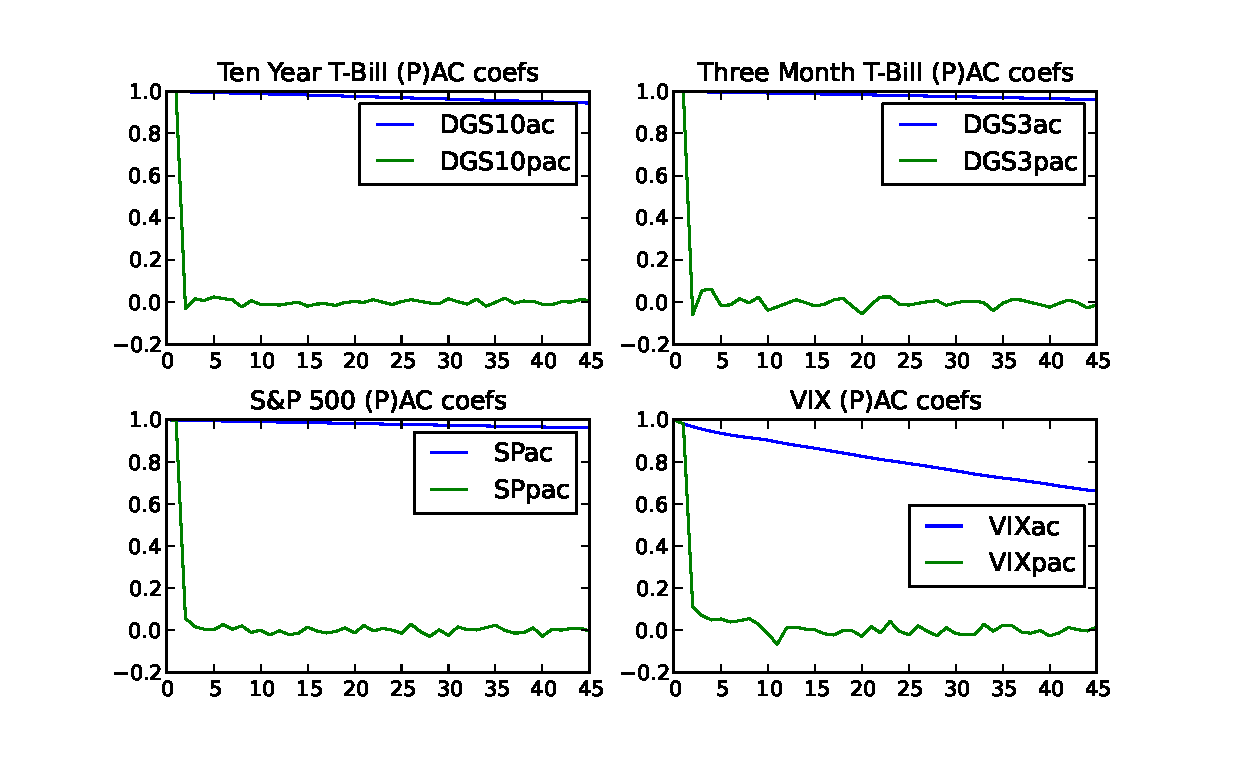
\includegraphics[width=6in]{./Figures/all_corrs.eps}
        \captionsetup{width=5.5in}
        \caption{\small Autocorrelation and partial autocorrelation coefficients for each data set. Used to find the parameters $q$ and $p$ in an ARIMA model. The initial spike in the partial autocorrelation coefficients and the gradual descent of the autocorrelation coefficients suggets $p=1$, and $q=0$.}
        \label{fig:correlations}
      \end{figure}

      As can be clearly seen, for each of my time series we have an initial spike in the partial autocorrelation coefficient for 1 lag and then nothing. Also, in each picture we see that the autocorrelation coefficients slowly decline for all 4 time series. Together, these two pieces of information suggest that we should approximate an AR(1) model by setting $p = 1 $and $q = 0$. Another important feature in each of this plots is that while the decrease in the autocorrelation coefficients is steady, it is also very slow. This is indicative of a need to difference the data to make it more stationary before applying the model.

      The last identification step is to determine a suitable value for d, or determine how many times the data needs ot be differenced before it is stationary. This is a bit more subjective, but can still be formalized. I used two different techniques to do this. The first was taking successive differences of the data, looking at plots and the first two moments and stopping when the data looks stationary.  In Table~\ref{tab:differences} I have included a table that reports the mean and variance of the first 4 differences for all 4 data sets.

      \begin{table}
        \begin{centering}
        \setstretch{1.25}
        \begin{tabular}{|l|c|cc||l|c|cc|}
          \hline
           \rowcolor{gray!45} DataSet & Lags &   Mean &     Variance & DataSet & Lags &   Mean &     Variance \\
          \hline
          \hline
           \rowcolor{gray!7} DGS10  & 1    & -0.0014 &  0.0039 & SP500  & 1    &   0.0344 &  224.2908 \\
           \rowcolor{gray!23} {} &     2    & -0.0028 &  0.0079 & {} &     2    &   0.0839 &  406.3557 \\
           \rowcolor{gray!7} {} &     3    &  -0.0042 &   0.0115 & {} &      3    &    0.1329 &   574.528 \\
           \rowcolor{gray!23} {} &     4    & -0.0056 &   0.0151 & {} &     4    &    0.1779 &  748.1064 \\
           \rowcolor{gray!7} DGS3MO &  1    & -0.0016 &  0.0033 & VIX    & 1    & -0.0034 &   3.1320 \\
           \rowcolor{gray!23} {} &     2    & -0.0032 &  0.0077 & {} &     2    & -0.0076 &  5.3557 \\
           \rowcolor{gray!7} {} &     3    &  -0.0048 &   0.0114 & {} &     3    &  -0.0118 &  7.2619 \\
           \rowcolor{gray!23} {} &     4    & -0.0064 &   0.0140 & {} &     4    &  -0.0154 &  9.0184 \\
          \hline
        \end{tabular}
        \setstretch{1.75}
        \captionsetup{width=5.5in}
        \caption{Mean and Variance of data sets for first 4 lags for each time series. The goal is stationarity, so the correct number of lags will have a small mean and variance.}
        \label{tab:differences}
        \end{centering}
      \end{table}

      The second method for determining the correct number of lags is to use an augmented Dickey Fuller test.  the augmented Dickey Fuller (ADF) test is used to check for unit roots in a time series. In other words, ADF is applied to a time series to see if the coefficient ends up being 1 when a time series is regressed on its lag. The null hypothesis in the ADF test is that there is a unit root. I performed the ADF for all four data sets for the data by itself as well as the first lag. The results appear in Table ~\ref{tab:dickeyfuller}.

      \begin{table}
        \begin{centering}
        \setstretch{1.25}
          \begin{tabular}{|l|l|cc|}
          \hline
            \rowcolor{gray!45} DataSet & Lags &  Statistic & p-value\\
            \hline
            \hline
            \rowcolor{gray!7} SP500 & 0 & -1.8564 & 0.6391\\
           \rowcolor{gray!23} {} & 1  & -18.0968 & 0.0001\\
            \rowcolor{gray!7} VIX & 0 & -4.9092 & 0.0001\\
           \rowcolor{gray!23} {} & 1  & -19.162 & 0.0001\\
            \rowcolor{gray!7} DGS10 & 0 & -3.9125 & 0.0133\\
            \rowcolor{gray!23} {} & 1 & -16.5723 & 0.0001\\
            \rowcolor{gray!7} DGS3MO & 0 & -1.5736 & 0.7589\\
            \rowcolor{gray!23} {} & 1 & -17.1829 & 0.0001\\
          \bottomrule
          \end{tabular}
          \setstretch{1.75}
          \captionsetup{width=5.5in}
          \caption{Results from the augmented Dickey-Fuller test. The test was run for each data set with no lags and again with a single lag. The test statistic corresponding to the 5\% confidence level is $ -3.5$. Any statistic lower than that suggests that the data might already be stationary (hence the small p-value).}
          \label{tab:dickeyfuller}
        \end{centering}
      \end{table}

      \begin{figure}[!h]
        \centering
        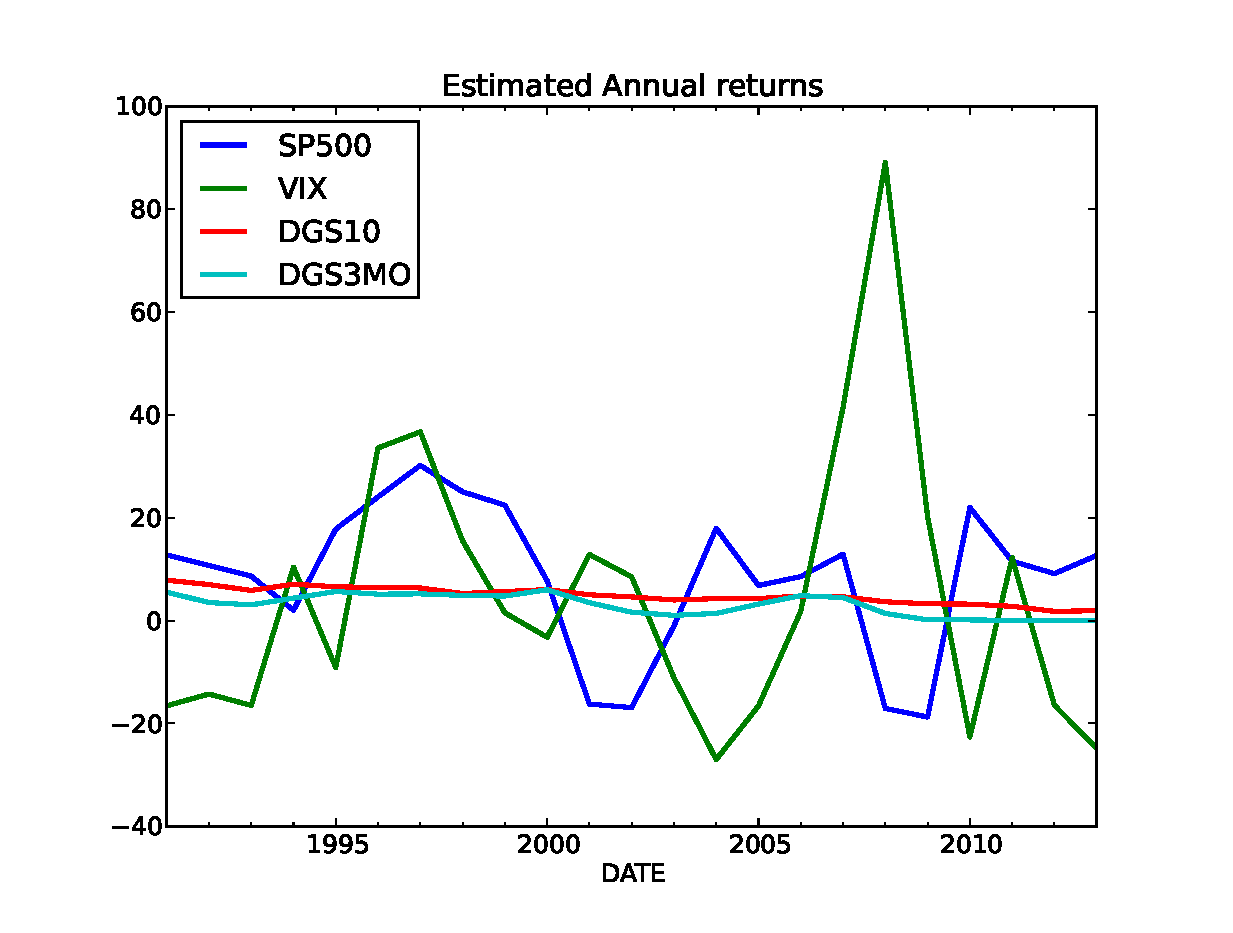
\includegraphics[width=6in]{./Figures/returns.eps}
        \captionsetup{width=5.5in}
        \caption{\small Average (estimated) annual returns for the S\&P 500, VIX, DGS10, and DGS3MO time series from 1991 to 2012.}
        \label{fig:returns}
      \end{figure}

  \subsection{(G)ARCH Models} \label{sub:garch}

\section{Forecasting} \label{sec:forecasting}

\section{Estimating Returns} \label{sec:estimatingreturns}

\section{Conclusion} \label{sec:conclusion}

\newpage

\bibliography{EPP_TSA}

\end{document}
